\documentclass[12pt,twoside]{article}
%%%%%%%%%%%%%%%%%%%%%%%%%%%%%%%%%%%%%%%%%%%%%%%%%%%%%%%%%%%%%
% Meta informations:
\newcommand{\trauthor}{Jan Fabian Schmid}
\newcommand{\trtype}{Seminar Paper} %{Seminararbeit} %{Proseminararbeit}
\newcommand{\trcourse}{Bio-inspired Artificial Intelligence}
\newcommand{\trtitle}{Effects of encoding on the general learning ability of neural networks}
\newcommand{\trmatrikelnummer}{6440383}
\newcommand{\tremail}{2schmid@informatik.uni-hamburg.de}
\newcommand{\trarbeitsbereich}{Knowledge Technology, WTM}
\newcommand{\trdate}{11.11.2015}

%%%%%%%%%%%%%%%%%%%%%%%%%%%%%%%%%%%%%%%%%%%%%%%%%%%%%%%%%%%%%
% Languages:

% Falls die Ausarbeitung in Deutsch erfolgt:
% \usepackage[german]{babel}
% \usepackage[T1]{fontenc}
% \usepackage[latin1]{inputenc}
% \usepackage[latin9]{inputenc}	 				
% \selectlanguage{german}

% If the thesis is written in English:
\usepackage[english]{babel} 						
\selectlanguage{english}

%%%%%%%%%%%%%%%%%%%%%%%%%%%%%%%%%%%%%%%%%%%%%%%%%%%%%%%%%%%%%
% Bind packages:
\usepackage{acronym}                    % Acronyms
\usepackage{algorithmic}								% Algorithms and Pseudocode
\usepackage{algorithm}									% Algorithms and Pseudocode
\usepackage{amsfonts}                   % AMS Math Packet (Fonts)
\usepackage{amsmath}                    % AMS Math Packet
\usepackage{amssymb}                    % Additional mathematical symbols
\usepackage{amsthm}
\usepackage{booktabs}                   % Nicer tables
%\usepackage[font=small,labelfont=bf]{caption} % Numbered captions for figures
\usepackage{color}                      % Enables defining of colors via \definecolor
\definecolor{uhhRed}{RGB}{254,0,0}		  % Official Uni Hamburg Red
\definecolor{uhhGrey}{RGB}{122,122,120} % Official Uni Hamburg Grey
\usepackage{fancybox}                   % Gleichungen einrahmen
\usepackage{fancyhdr}										% Packet for nicer headers
%\usepackage{fancyheadings}             % Nicer numbering of headlines

%\usepackage[outer=3.35cm]{geometry} 	  % Type area (size, margins...) !!!Release version
%\usepackage[outer=2.5cm]{geometry} 		% Type area (size, margins...) !!!Print version
%\usepackage{geometry} 									% Type area (size, margins...) !!!Proofread version
\usepackage[outer=3.15cm]{geometry} 	  % Type area (size, margins...) !!!Draft version
\geometry{a4paper,body={5.8in,9in}}

\usepackage{graphicx}                   % Inclusion of graphics
%\usepackage{latexsym}                  % Special symbols
\usepackage{longtable}									% Allow tables over several parges
\usepackage{listings}                   % Nicer source code listings
\usepackage{multicol}										% Content of a table over several columns
\usepackage{multirow}										% Content of a table over several rows
\usepackage{rotating}										% Alows to rotate text and objects
\usepackage[hang]{subfigure}            % Allows to use multiple (partial) figures in a fig
%\usepackage[font=footnotesize,labelfont=rm]{subfig}	% Pictures in a floating environment
\usepackage{tabularx}										% Tables with fixed width but variable rows
\usepackage{url,xspace,boxedminipage}   % Accurate display of URLs

%%%%%%%%%%%%%%%%%%%%%%%%%%%%%%%%%%%%%%%%%%%%%%%%%%%%%%%%%%%%%
% Configurationen:

\hyphenation{whe-ther} 									% Manually use: "\-" in a word: Staats\-ver\-trag

%\lstloadlanguages{C}                   % Set the default language for listings
\DeclareGraphicsExtensions{.pdf,.svg,.jpg,.png,.eps} % first try pdf, then eps, png and jpg
\graphicspath{{./src/}} 								% Path to a folder where all pictures are located
\pagestyle{fancy} 											% Use nicer header and footer

% Redefine the environments for floating objects:
\setcounter{topnumber}{3}
\setcounter{bottomnumber}{2}
\setcounter{totalnumber}{4}
\renewcommand{\topfraction}{0.9} 			  %Standard: 0.7
\renewcommand{\bottomfraction}{0.5}		  %Standard: 0.3
\renewcommand{\textfraction}{0.1}		  	%Standard: 0.2
\renewcommand{\floatpagefraction}{0.8} 	%Standard: 0.5

% Tables with a nicer padding:
\renewcommand{\arraystretch}{1.2}

%%%%%%%%%%%%%%%%%%%%%%%%%%%%
% Additional 'theorem' and 'definition' blocks:
\theoremstyle{plain}
\newtheorem{theorem}{Theorem}[section]
%\newtheorem{theorem}{Satz}[section]		% Wenn in Deutsch geschrieben wird.
\newtheorem{axiom}{Axiom}[section] 	
%\newtheorem{axiom}{Fakt}[chapter]			% Wenn in Deutsch geschrieben wird.
%Usage:%\begin{axiom}[optional description]%Main part%\end{fakt}

\theoremstyle{definition}
\newtheorem{definition}{Definition}[section]

%Additional types of axioms:
\newtheorem{lemma}[axiom]{Lemma}
\newtheorem{observation}[axiom]{Observation}

%Additional types of definitions:
\theoremstyle{remark}
%\newtheorem{remark}[definition]{Bemerkung} % Wenn in Deutsch geschrieben wird.
\newtheorem{remark}[definition]{Remark} 

%%%%%%%%%%%%%%%%%%%%%%%%%%%%
% Provides TODOs within the margin:
\newcommand{\TODO}[1]{\marginpar{\emph{\small{{\bf TODO: } #1}}}}

%%%%%%%%%%%%%%%%%%%%%%%%%%%%
% Abbreviations and mathematical symbols
\newcommand{\modd}{\text{ mod }}
\newcommand{\RS}{\mathbb{R}}
\newcommand{\NS}{\mathbb{N}}
\newcommand{\ZS}{\mathbb{Z}}
\newcommand{\dnormal}{\mathit{N}}
\newcommand{\duniform}{\mathit{U}}

\newcommand{\erdos}{Erd\H{o}s}
\newcommand{\renyi}{-R\'{e}nyi}
%%%%%%%%%%%%%%%%%%%%%%%%%%%%%%%%%%%%%%%%%%%%%%%%%%%%%%%%%%%%%
% Document:
\begin{document}
\renewcommand{\headheight}{14.5pt}

\fancyhead{}
\fancyhead[LE]{ \slshape \trauthor}
\fancyhead[LO]{}
\fancyhead[RE]{}
\fancyhead[RO]{ \slshape \trtitle}

%%%%%%%%%%%%%%%%%%%%%%%%%%%%
% Cover Header:
\begin{titlepage}
	\begin{flushleft}
		Universit\"at Hamburg\\
		Department Informatik\\
		\trarbeitsbereich\\
	\end{flushleft}
	\vspace{3.5cm}
	\begin{center}
		\huge \trtitle\\
	\end{center}
	\vspace{3.5cm}
	\begin{center}
		\normalsize\trtype\\
		[0.2cm]
		\Large\trcourse\\
		[1.5cm]
		\Large \trauthor\\
		[0.2cm]
		\normalsize Matr.Nr. \trmatrikelnummer\\
		[0.2cm]
		\normalsize\tremail\\
		[1.5cm]
		\Large \trdate
	\end{center}
	\vfill
\end{titlepage}

	%backsite of cover sheet is empty!
\thispagestyle{empty}
\hspace{1cm}
\newpage

%%%%%%%%%%%%%%%%%%%%%%%%%%%%
% Abstract:

% Abstract gives a brief summary of the main points of a paper:
\section*{Abstract}
  Your text here...

% Lists:
\setcounter{tocdepth}{2} 					% depth of the table of contents (for Seminars 2 is recommented)
\tableofcontents
\pagenumbering{arabic}
\clearpage

%%%%%%%%%%%%%%%%%%%%%%%%%%%%
% Content:

% the actual content, usually separated over a number of sections
% each section is assigned a label, in order to be able to put a
% crossreference to it

\section{Introduction}
\label{sec:introduction}

The studied paper: \cite{citeulike:12788284}\\
What research question is examined in the paper?\\
Solution suggested by this paper?\\
\textbf{My Research question for the in-depth analysis:}\\
- What effect has the usage of different neural net encodings on neural plasticity?

\section{related work}
Typical approaches from related work\\
- typically the two problems ( 1. encoding of nervous systems for evolution of large good neural networks and 2. synaptic plasticity in neural networks) are studied separately\\
About generative encodings: \\
- \cite{hornby2001body} $\rightarrow$ L-Systems\\
- \cite{mouret2010importing} $\rightarrow$ neuroscience toolbox\\
About synaptic plasticity:\\
- \cite{hebb2005organization} $\rightarrow$ importance of synaptic plasticity for learning\\
- \cite{abbott2000synaptic} $\rightarrow$ synaptic plasticity in neural networks

\section{Background Information}
\label{sec:background}

From genes to nervous systems\\
- Direct and developmental encodings\\
Skinner-box\\
- Where and for what purpose can this experiment be used?\\
Definition of regularity used in this paper\\
Different encodings to describe neural networks tested in this paper\\
- How do they work?\\
- What differentiates them?


\subsection{map-based encoding}
The map-based encoding develops a network structure in a similar way as the direct encoding does, but instead of directly setting neurons and their connections, nodes and edges are used.
Nodes and Edges of the developed neural net are however encoded in a specific, more complex way. Because of this part of the encoding it doesn't behave as a direct encoding, but as a developmental encoding.\\
Each node of the network represents a whole map of neurons. A map of neurons is an array of $N \times M$ identical neurons and is defined by a set of parameters (??? \cite{tonelli2011using} p. 3). 
In the map-based encoding in the studied paper each parameter value is a real number between 0 and 1 and is mutated during the evolutionary process.
The meaning of an parameter 'flips' by exceeding a certain value (for example: a parameter value between 0 and 0.4 means 'a' and between 0.4 and 1 'b').
One parameter of the neuron map for example decides if it represents only a single neuron or a set array size of neurons.\\
The edges between maps are described as well with a number of parameters.
In this case the type of connection and the synaptic weight are set by parameters.
One parameter decides if each neuron of a map is only connected to one neuron of the map on the other side of the edge or if each neuron is connected to each other neuron.
Another parameter implies if the connection weights have positive or negative sign (excitatory or inhibitory). And the last parameter sets the weight value.

\subsection{HNN encoding}
The Hyper Neural Network (HNN) encoding used by Tonelli and Mouret is a modification of the complex HyperNEAT encoding.
When using this encoding the network structure has to be specified beforehand (in this case 9 input neurons, 5 hidden neurons and 4 output neurons).
During the evolutionary development of the network two additional included networks are formed. One of them answers the question to each pair of neurons, if they are connected or not and if so which connection weight the edge has.
The second inherent network defines the parameters of each neuron. These two networks are developed using the direct encoding.
Through the interaction of the two inherent networks with the given main-network structure a the HNN encoding meets the requirements of a developmental encoding.

\subsection{Skinner box}
A Skinner box is a typical experiment to test the learning ability of an animal (usually rats).
The standard configuration of a Skinner box can be seen in figure \ref{fig:skinner}, it can be described with input and output items.
The test animal has to associate the inputs with the	appropriate output.
As main input, lights or sounds from a loudspeaker might be used. The test animal is then supposed to press the associated response lever according to the input pattern.
The association patterns are set arbitrarily by the experimenter. For example the test animal might be supposed to push the lever (as output) if the green light appears, but not if the red light shines.
As additional input the food dispenser and electrified grid can then be used to support the 'right' behaviour and/or punish the 'wrong' behaviour.

\begin{figure}[h]
	\begin{center}
		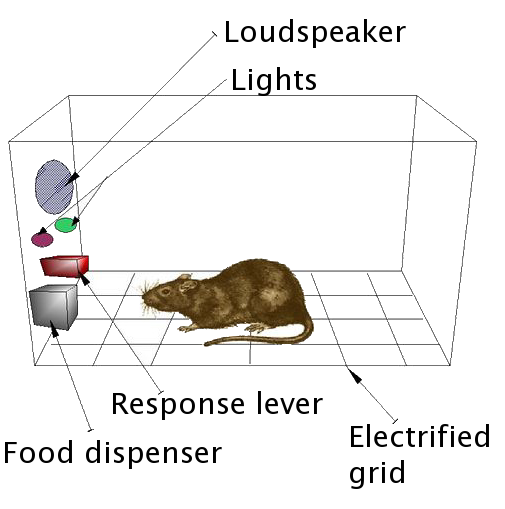
\includegraphics[width=.43\textwidth]{Skinner_box_scheme_01.png}
	\end{center}
	\caption{Skinner box, wiki}
	\label{fig:skinner}
\end{figure}

A test animal (or different test object) with good general learning ability, should be able to identify the supported input to output associations independent of the specific used pairing and act accordingly.

\section{Approach description}
\label{sec:model}
Proposal of the paper\\
- Bias towards regularity is critical to evolve plastic neural networks\\
Experiment in the paper to verify the proposal\\
- How is it structured?\\
- What is it able to show?\\
- Expected results?\\

\section{Approach analysis}
\label{sec:analysis}

Results from the presented experiment\\
- Are the results according to the proposal?\\
Which effects did the different encodings have?\\
- Map-based encoding\\
- HNN\\
- Direct encoding\\
Critique\\
- Were the choosen encodings reasonable and sufficient?\\

%psychological consistence of results\\
%- importance of regularity\\
%\cite{Hornby:2002:AL}\\
%\cite{journals/tec/CluneSPO11}\\

%- variability selection\\
%\cite{potts1998variability}\\
%- optimal fully connected brain\\
%- synaptic plasticity\\
%\cite{abbott2000synaptic}\\
%\cite{yang2014sleep} $\rightarrow$ synaptic plasticity important for learning and memory\\

\section{Conclusion}
\label{sec:concl}

How reasonable is the approach of the paper?\\
General conclusions about the effect of different encodings for neural networks\\

%%%%%%%%%%%%%%%%%%%%%%%%%%%%%%%%%%%%%%
% hier werden - zum Ende des Textes - die bibliographischen Referenzen
% eingebunden
%
% Insbesondere stehen die eigentlichen Informationen in der Datei
% ``bib.bib''
%
\newpage
\bibliographystyle{plain}
\addcontentsline{toc}{chapter}{Bibliography}% Add to the TOC
\bibliography{bib}

\end{document}


